\section{Implementation choices}
In this section we describe the proposed architecture in more detail. We present the excerpt on the internal structure of both public and private chains and the reasoning behind these choices.

In order to deduce the internal structure of our system, we first analyze its use-cases. The overview of the education process is given in Section~\ref{sec:architecture}. The communication between the Student and the Educator is saved as transactions in the private chain. However, the implementation details of this chain mostly depend on the data disclosure process.

We will start from analyzing this process and determining the main issues that arise from the need to disclose and verify the validity of the private blocks. Then we will propose the structure of the private and public blocks that addresses these issues.

\subsection{Anonymity and certification}
\label{sec:cert}
The permissionless nature of our public chain leads to the ability for malevolent students to create educational institutes in order to get the scores for the courses they did not attend. Moreover, the knowledge students actually get by completing the course, and the conditions upon which the course is considered completed, vary significantly between the educational institutions.

These issues currently can not be solved solely on the protocol level: they require an external source of information to determine the physical existence and the reputation of an Educator. Although we leave the public chain open for the Educators to submit their private block headers, we propose to add a separate layer of reputation and trust on top of the protocol.

We do so by introducing the Archivists -- the entities that join the network with the approval from another Archivist. Their main role is to add a trust level above just the raw protocol: they store the certificates of the Educational institutes and have the right to revoke those certificates. Furthermore, the Archivists are the entities responsible for determining the ratings of the particular Educators. The Archivists base their rating on the off-chain sources of information and gain authority for providing valid ratings and performing all the necessary compliance procedures for the Educators.

While in theory the Recruiters can query the Educators directly and initiate a data disclosure request, they are generally discouraged to do so. We expect the Recruiters to be willing to pay extra fees to the Archivists for certificate validation and ranking of the Students depending on the Educators' ratings and other factors upon request. We describe the data disclosure process in detail in section \ref{sec:DataDisclosure}

\subsection{Activity Type Graph}
\label{sec:ATG}
When a Recruiter makes a request to one of the Archivists, the Archivist has to somehow choose the relevant Educators. Moreover, when an Educator discloses the data, it has to provide as minimal set of entries as possible. This set has to be verifiable, which means that the Educator provides the proof of the data validity along with the data being disclosed.

In order to achieve these goals, we divide the data that the Educators store into atomic Activity Types. Each Educator maintains a journal of transactions per each Activity Type that the Educator offers.

All the Activity Types are grouped into courses that are further grouped into larger entities such as subjects and areas of knowledge. This grouping can be stored as the Activity Type Graph $G_A$ with the following properties:
\begin{enumerate}[label=\arabic*${}^\circ$]
\item $G_A$ is a directed graph:
  \begin{equation}
  G_A:\ \langle V: \{\mathrm{Vert}\},\ e_{out}: \mathrm{Vert} \rightarrow \{\mathrm{Vert}\}\ |\ \mathrm{rest} \rangle
  \end{equation}

\item Each vertex of $G_A$ is associated with depth:
  \begin{equation}
  G_A:\ \langle d: \mathrm{Vert} \rightarrow \mathrm{Int}\ |\ \mathrm{rest}  \rangle
  \end{equation}

\item Law of pointing down:
  \begin{equation}
  G_A:\ \langle v \in e_{out}(u) \implies d(v) > d(u) \rangle
  \end{equation}

\item $G_A$ has special \textit{et cetera} vertices $u$:
  \begin{equation}
  \forall\ v \in V\ \exists u\ (u \in e_{out}(v) \land e_{out}(u) = \emptyset)
  \end{equation}
\end{enumerate}

The example of the Activity Type Graph (ATG) is shown in Figure~\ref{fig:atg}. The vertex $v$ of the graph is a \textit{leaf} if $e_{out}(v) = \emptyset$. Otherwise we call it an \textit{internal vertex}. Every internal vertex of the graph has a special \textit{etc.} child (some of these are ommitted in the figure).

\begin{figure}[ht]
\centering
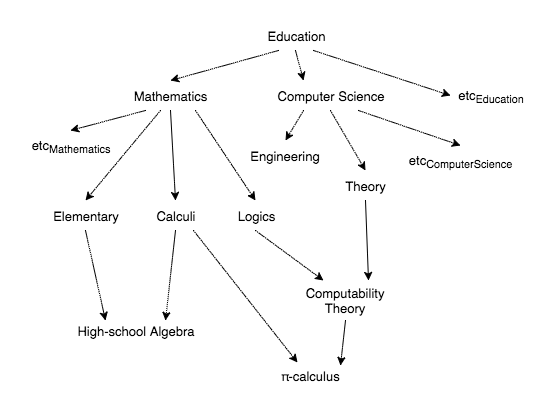
\includegraphics[width=0.8\textwidth]{atg}
\caption{An example of the Activity Type Graph. Some of the vertices are not shown}
\label{fig:atg}
\end{figure}

The need for \textit{etc.} vertices arises from the fact that not all of the Educators teach courses exactly in leaves — some of them offer general courses that provide just the necessary background. For example, some of the universities teach the basic \textquote{Computer science} course, that contains the basics of the discipline. In this case, when the particular category is hard to define, the university would use the $\textrm{etc}_{\textrm{ComputerScience}}$ vertex.

On the protocol level, the Educators can announce that they teach a particular course, but can not modify the Activity Type Graph structure. The structure of the graph is maintained by the core developers and updated upon request from the Educators.

\subsection{Search queries}

An educator can answer one of the following queries:
\begin{itemize}
\item For a set of pairs $(subjectId_1, minGrade_1)$, $(subjectId_2, minGrade_2)$, ..., $(subject_n, minGrade_n)$ and some $Count$, find no more than $Count$  students with grades satisfying the following inequalities:
\[
\left\{
\begin{array}{c}
avgGrade_{subjectId_1} >= minGrade_1 \\ avgGrade_{subjectId_2} >= minGrade_2 \\
\mathrel{\makebox[\widthof{=}]{\vdots}} \\ avgGrade_{subjectId_n} >= minGrade_n
\end{array}
\right.
\]

\item For the given identifier of a student, return all info about this student.
\item For given time range, activity and student, return hashes of work (merkle tree root) of assignments submitted. Returning a root will allow the opposite side of the trade to prove that transmitted data was corrupted without full public disclosure.
\end{itemize}

\subsection{Private chain}
\label{sec:priv-chain}

Every educator has a private chain. It stores the data about students, and can
generate answers for the queries described above.

Private chain comprises of two main data structures:
\begin{itemize}
\item Set of transactions batched into blocks. Every block contains a list of
  transactions packed into a Merkle tree.
\item Links to the transactions stored in the B+-tree with keys (studentId,
  studentGrade). Indexes constructed in such a way that more popular activities
  go first.
\end{itemize}

The structure of the private block is shown in Figure~\ref{fig:privateblocks}.
The block consists of a public \textit{header} that the Educators relay to the
Witnesses, and the private \textit{body} that remains in the educational
institute until it receives a data disclosure request.

\begin{figure}[ht]
\centering
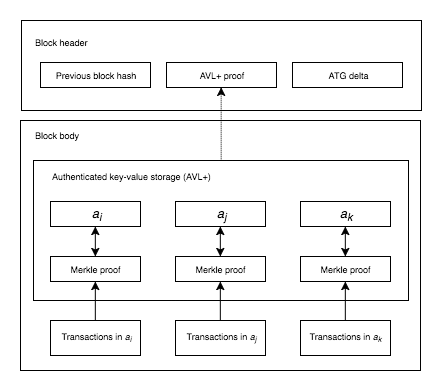
\includegraphics[width=0.8\textwidth]{private-blocks}
\caption{Private block structure}
\label{fig:privateblocks}
\end{figure}

During the educational process the Educators emit atomic \textit{private
  transactions}. These transactions represent the modifications to the journal of
academic achievements (thus, making a transaction means appending the data to
the journal). The transactions can be of the following types:

\begin{itemize}
\item student enrolls in a course;
\item student gets an assignment;
\item student submits an assignment;
\item student gets a grade for an assignment;
\item student gets a final grade for the course.
\end{itemize}

The first two types should be intiated by a student, and should include
student's signature to prevent spam from partially-honest educator. The
structure of the transaction is shown in Figure~\ref{fig:private-transactions}.

Let us denote an $i$-th transaction in a block as $T_{priv}^i$. The Educators
group the transactions that occured during the current block time slot, and
construct a Merkle tree \cite{merkle1989certified} for these journal
modifications:

\begin{equation}
M_{priv} = \MerkleTree(\{\ T_{priv}^i\ \})
\end{equation}

\begin{figure}[ht]
\centering
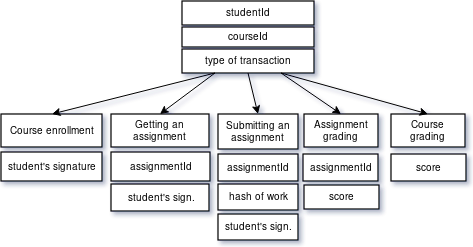
\includegraphics[width=0.8\textwidth]{private-transactions}
\caption{Transaction structure}
\label{fig:private-transactions}
\end{figure}

The Educator's private block body comprises an ordered set of
Merkle-authenticated transactions. These transactions are indexed so that the
Educator can quickly find a particular transaction that satisfies some
predicate.

The private block header consists of the transactions Merkle root along with the
previous block hash and the information on the Activity Type Graph modifications
(ATG delta). The \textit{ATG delta} part allows the Educators to inform the
Witnesses of the modifications to the courses they teach. The ATG delta is a
pair of sets $\Delta_A = (\Delta_{A+}, \Delta_{A-})$, where $\Delta_{A+}$ is a
set of subjects for which Educator starts a course and $\Delta_{A-}$ is a set of
subjects for which Educator closes a course.

An Educator collects private transactions into the blocks with no more than $K_{max}$
transactions per each block. After that, an Educator submits signed block header
to the Witnesses so that private transactions can be confirmed by the public
chain. Thus, the private blocks form a publicly verifiable chain of events.

\begin{figure}[ht]
\centering
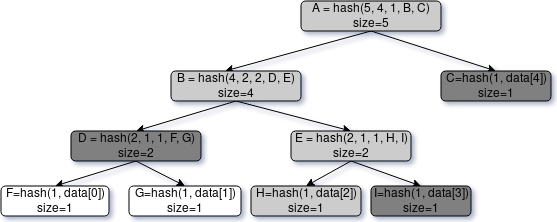
\includegraphics[width=0.7\textwidth]{merkle-tree}
\caption{Example of sized Merkle tree}
\label{fig:merkle-tree}
\end{figure}

To incentivize Witnesses to include private block headers into the public chain,
an Educator should pay some amount of coins per each private block. We should
take into consideration that an educator may be both a local tutor and some big
university. Depending on that, a number of transactions per each block, as well
as paying capacity, may differ. So the cost of a digest publication should
linearly grow with the size of a block. Let the cost for publishing a
public block header be
\begin{equation}\label{sec:priv-chain:pub-cost-eq}
  C_{pub}(B) = \alpha_{pub} + \beta_{pub} \cdot N_{tr}(B)
\end{equation}
, where $N_{tr}(B)$ is the number of transactions in private block $B$ and
$\alpha_{pub}$ and $\beta_{pub}$ are parameters of the network -- a small
constant fee and a linear price coefficient accordingly.

From the description above we can conclude that an educator may have an incentive to lie about the size of the tree. To achieve the ability to prove the number of transactions in the Merkle tree,
we will store the size of the subtree with the hash in each node (as shown in \ref{fig:merkle-tree}). So every transaction disclosure will also verify the size. Suppose that an Educator published a header hash with a wrong size, then every student which is collecting his own fair CV will see that an Educator deceives him, and moreover not a single data-disclosure deal would proceed.

Let's look at the example from the figure \ref{fig:merkle-tree}. Suppose we need to disclose $data[2]$. The path to the node H is $A \rightarrow B \rightarrow E \rightarrow H$. The proof nodes are $C$, $D$, and $I$. So the size of the tree is $$C.size+D.size+I.size+1=5$$


We also consider a possibility for small educators to form pools and release
blocks together in order to reduce costs for each individual educator. See
appendix \ref{apx:pools} for details.

\subsection{Public chain}
The Witnesses maintain a public chain -- a distributed ledger that contains publicly available information. If one wishes to perform a transaction on the public chain, she has to pay a certain fee that serves two purposes. First of all, the fee incentivizes the Witnesses to participate in the network and issue new blocks. Second, by requiring a fee for each transaction, we protect the public ledger from being spammed.

We present the structure of the public blocks in Figure~\ref{fig:publicblocks}. The public ledger contains the following information:
\begin{enumerate}
\item Modification history of the Activity Type Graph.
\item Private transaction proofs.
\item Account balances and value transfer history.
\end{enumerate}

\begin{figure}[ht]
\centering
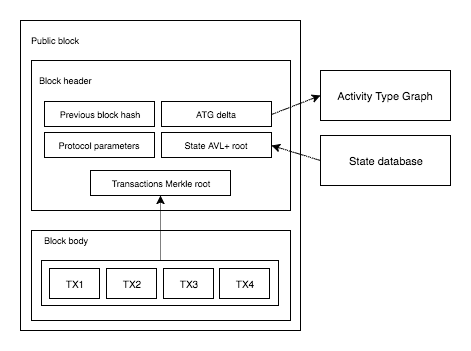
\includegraphics[width=0.8\textwidth]{public-blocks}
\caption{Public block structure}
\label{fig:publicblocks}
\end{figure}

There are two major ways to store the account balances and other state information: UTXO and account-based architectures. UTXO is an unspent transaction output, that contains some predicate -- a condition that has to be fulfilled in order to spend the coins. To prove the money ownership, the spender provides a witness -- an input that makes the predicate true. Thus, the UTXO-based architecture requires the transactions to be stateless, effectively limiting the application domain \cite{bentov2017instantaneous}.  The unspent outputs with an associated state can be treated as smart-contracts in the account-based architectures like Ethereum \cite{wood2014ethereum}. The state is stored in an off-chain storage -- the state database. The transactions are treated as the modifications of the world state.

Disciplina uses an account-based ledger with contracts programmable in Plutus language \cite{Plutus}. Each account has an associated state, which comprises the account balance and other information (e. g. log $L$ of a data disclosure contract). The world state is a mapping between accounts and their states. In order to make this mapping easily verifiable, we use a structure called the \textit{authenticated AVL+ tree} introduced in~\cite{reyzin2016improving}. This structure is based on state-of-the-art research that enables for faster verification of the mapping and allows us to never disclose it: the Witnesses would not have to store the whole blockchain like Bitcoin or Ethereum nodes do. Rather, they would just have to check the private block headers in order to confirm that none of the private blocks were tampered with.

The recent achievements in the field of consensus protocols, like the provably secure Ouroboros \cite{kiayias2017ouroboros}, allow us to build a public chain based on the Proof of Stake consensus rules. Thus, we can increase the transaction speed and drop the need for the expensive mining. However, with mining being dropped, we need to provide incentives for the Witnesses to maintain the chain and participate in the network.

% \subsection{Incentives}

In order to incentivize the Witnesses as well as the Archivists and the Object Store maintainers we propose a monetary policy with two main sources of income. The first one is the technical pool — a special pool of tokens, which are reserved until the participants acquire them through contributions to the operation of the platform. The tokens from the technical pool will be distributed with exponential slowdown. Running the nodes for different entities of the system require different hardware resources and there may come a point where the system lacks the nodes of a certain entity. To overcome this issue, the complexity and the amount of tokens received by the participants will be determined dynamically so that the equilibrium between the entities is preserved, for example, if the system lacks the Archivists, the incentive to run the Archivist's node would be more then the one for the Witnesses.

The second source of the participants' income is the fees for the transactions in the system. The Recruiters' fee is distributed among all the participants except the Object Store maintainers. The latter obtain tokens from the Educators paying them for the storage they offer.

\subsection{Fair CV}
\label{sec:fair-cv}
One of the main goals of the Disciplina platform is to provide a way for the Students to easily prove their educational records. We propose to duplicate the records in the Student's \textit{digital CV.} This CV contains all the records that the parties have generated during the Student's educational process along with the validity proofs of that data (see Figure~\ref{fig:cv}).

\begin{figure}[ht]
\centering
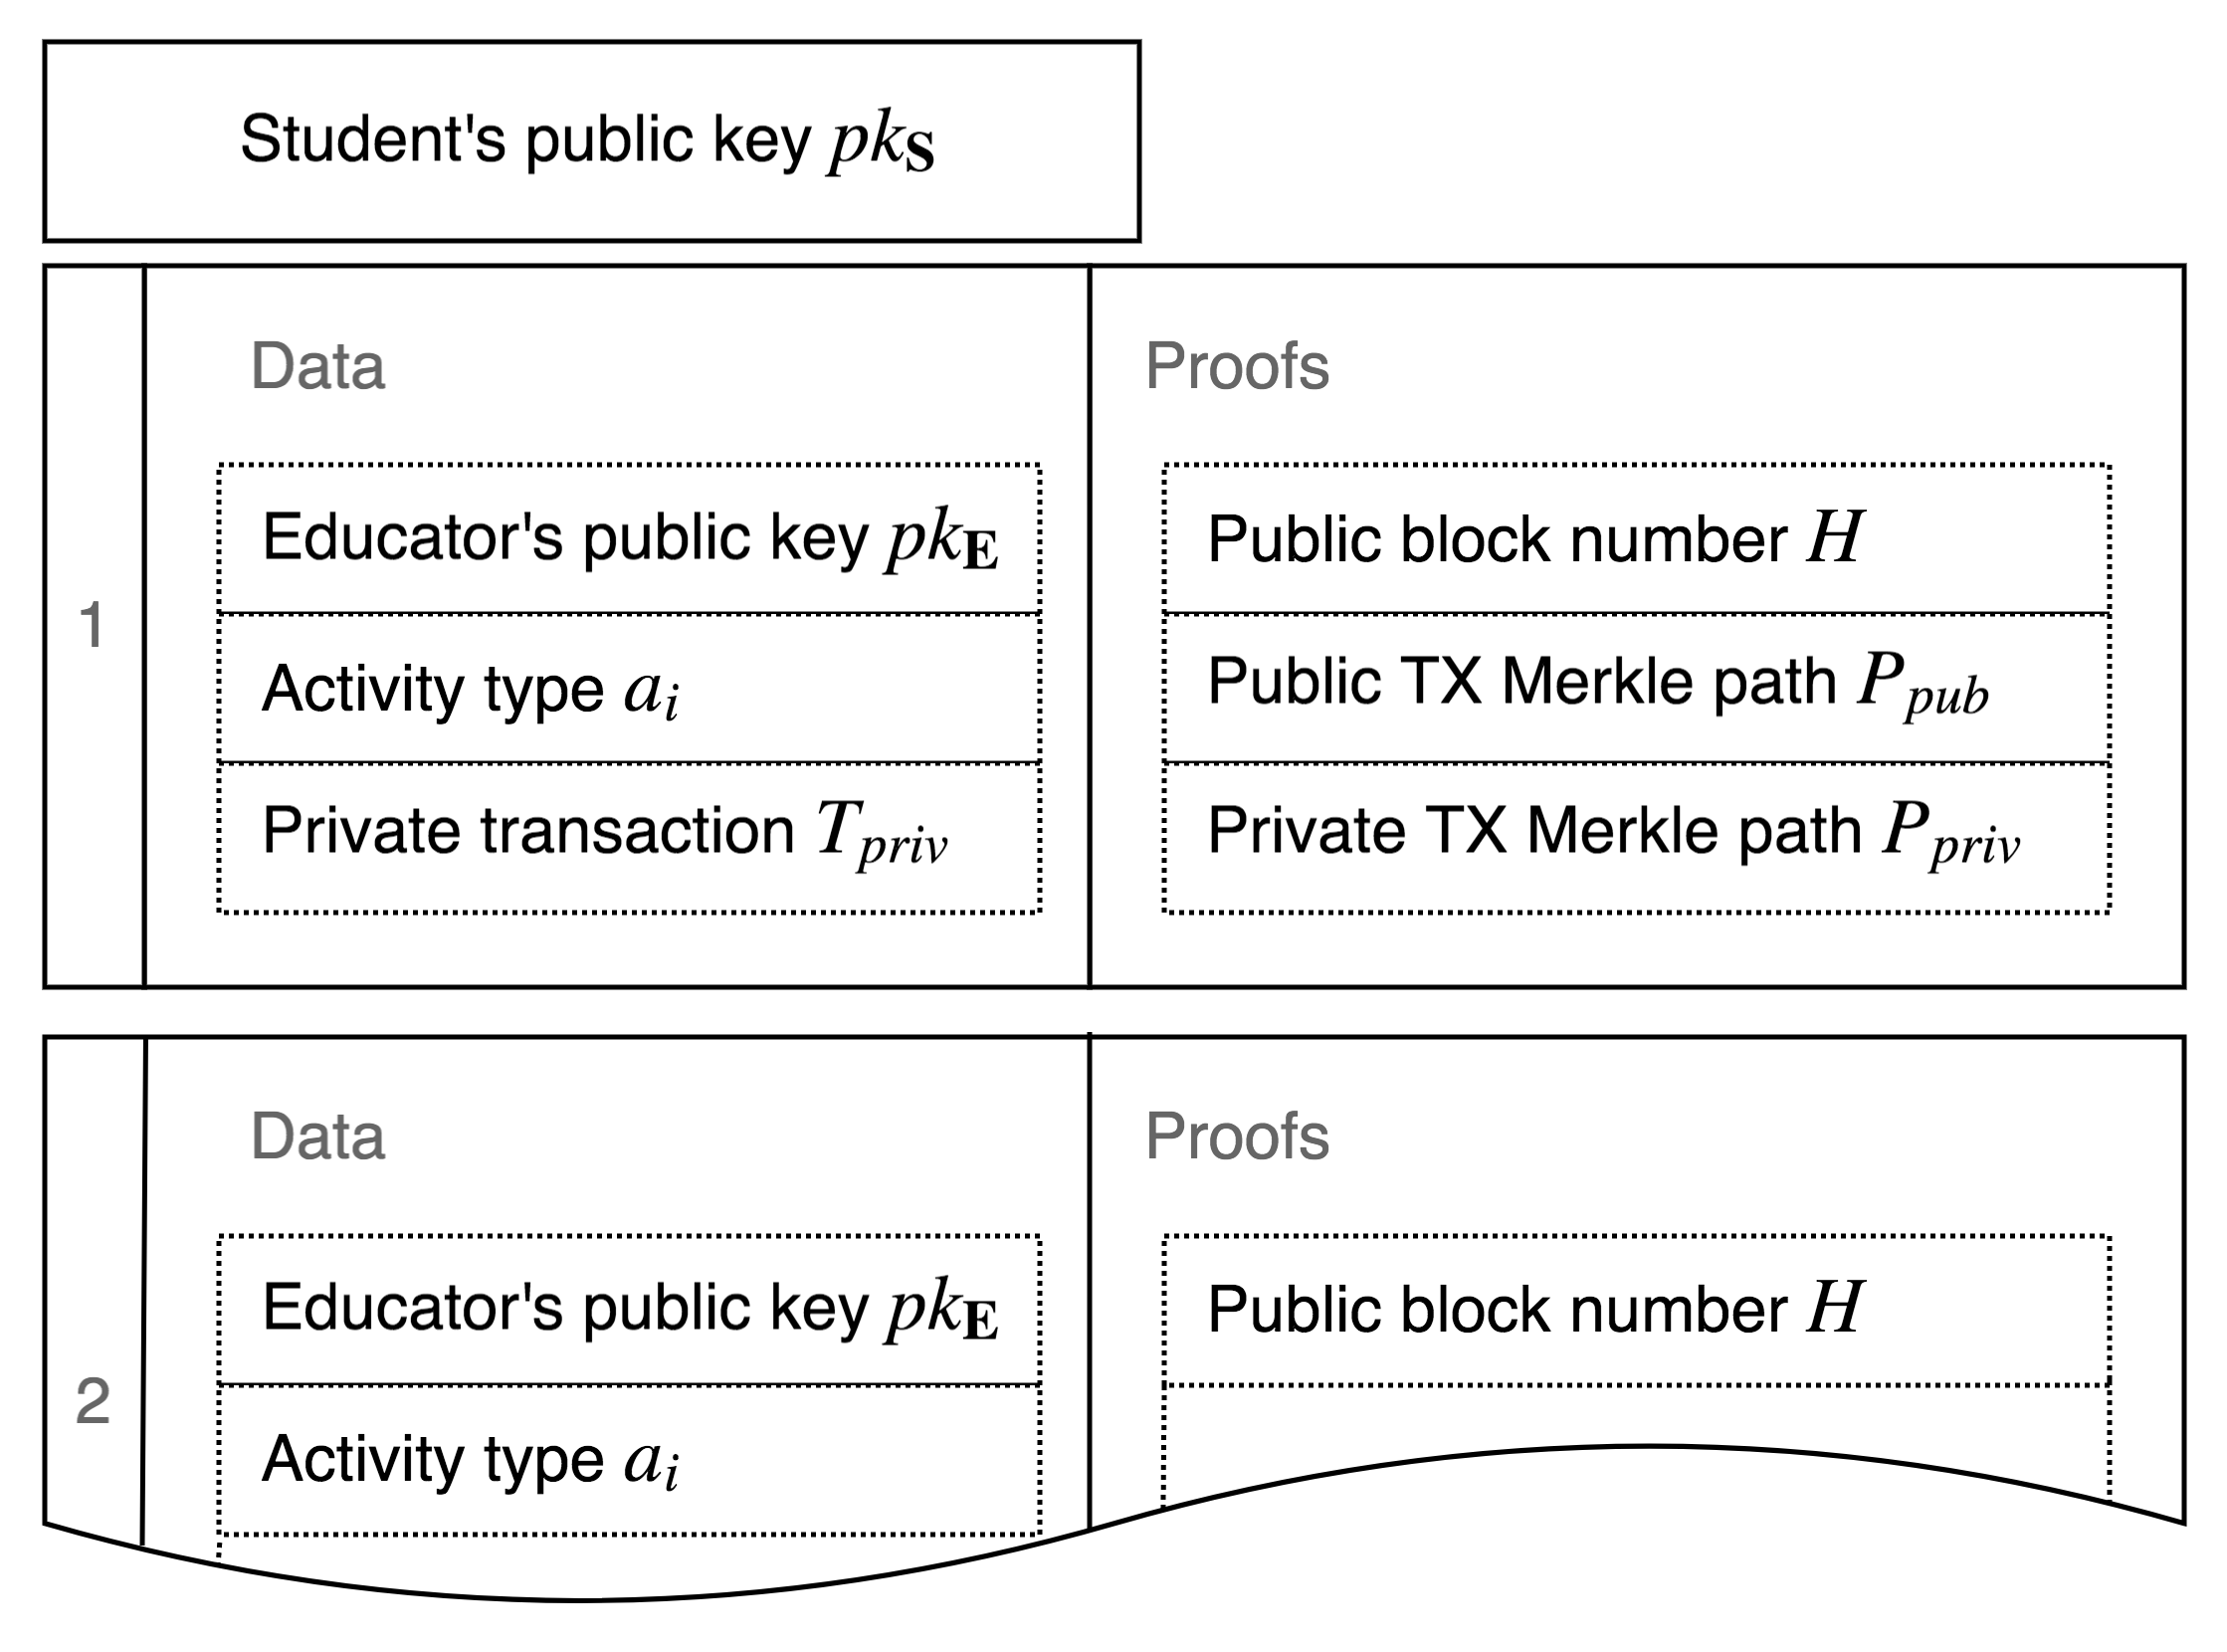
\includegraphics[width=0.8\textwidth]{cv}
\caption{Student's authenticated CV}
\label{fig:cv}
\end{figure}

In order to prove that some transaction actually occurred in some private block of the concrete Educator, the student has to provide the cryptographic proofs along with the actual data. The cryptographic proof of the inclusion of an element in an authenticated data structure is generally a path of hashes. Let us denote the path of the element~$e$ in some authenticated data structure~$X$ as~$\Path(e, X)$. Thus, the Student has to  provide the following data:
\begin{itemize}
  \item The Student's and the Educator's public keys $\PubKey{S}$ and $\PubKey{E}$.
  \item The course $a_i$ and the a private transaction $T_{priv}$ with the score.
  \item The Merkle path of the transaction in the journal: $P_{priv} = \Path(T_{priv}, M_{priv})$, where $M_{priv}$ is a Merkle tree of the transactions in the private block.
  \item The public block number $H$ and the Merkle path of the transaction $T_{pub}$ that pushed the private block into the public chain: $P_{pub} = \Path(T_{pub}, M_{pub})$, where $M_{pub}$ is a Merkle tree of the transactions in the block $H$.
\end{itemize}

Having this data one can prove the occurrence of a certain transaction in one of the Educator's private blocks without the need to request any data from the Educator during the validation process. Thus, any party can check the validity of the Student's CV for free if the Student wishes to disclose it.

Let $\rho(e, P)$ be the function that substitutes the element $e$ in path $P$ and computes the root hash of the authenticated data structure. Then the validation process is as follows:
\begin{enumerate}
\item Query the public chain to find the block $H$ and obtain the Merkle root of the transactions: $\Root(M_{pub})$.
\item Check whether $\rho(T_{pub}, P_{pub}) = \Root(M_{pub})$.
\item Check that the public transaction $T_{pub}$ was signed with the Educator's public key $\PubKey{E}$.
\item From the public transaction $T_{pub}$ obtain the Merkle root of the private transactions: $\Root(M_{priv})$.
\item Check that $\rho(T_{priv}, P_{priv}) = \Root(M_{priv})$.
\end{enumerate}

These validation steps can prove that an Educator with a public key $\PubKey{E}$ issued a transaction $T_{priv}$ in one of its private blocks. One can attribute the $\PubKey{E}$ to a particular real-world educational institution by checking the Educator's certificate as described in Section~\ref{sec:cert}.

\subsection{Data Disclosure}
\label{sec:DataDisclosure}
The process of data disclosure involves direct communication between a particular Educator, willing to disclose a part of the data, and an interested party~\tParty{B} (e. g. a recruiter), willing to pay for this data. Suppose an Educator~\tParty{E} has some data~$D$. To mitigate the risk of secondary market creation, one should ensure that the majority of the data remains in the private blocks. We propose to increase the cost of the data exponentially to its size, thus incentivizing the buyers to make as accurate requests as possible.

 Before the deal \tParty{E} ought to perform some preparation steps. \tParty{E} should:
\begin{enumerate}
\item Divide~$D$ into $N$ chunks of size no more than 1~KiB:

\begin{equation}
D = \Concat_{i=1}^N d_i, \quad \SizeOf(d_i) \leq 1~\mathrm{KiB}
\end{equation}

\item Generate a symmetric key $k$
\item Encrypt each~$d_i$ with $k$ and make an array of encrypted chunks:
\begin{equation}
\Lock{D} = \{ \Encrypt_\Key{k}(d_1),\ \Encrypt_\Key{k}(d_2),\ ...,\ \Encrypt_\Key{k}(d_N) \}
\end{equation}

\item Compute a Merkle root of the encrypted chunks:
\begin{equation}
R = \Root(\MerkleTree(\Lock{D}))
\end{equation}

\item Determine the size of the data she is going to reveal:
\begin{equation}
s = \SizeOf(\Lock{D})
\end{equation}

\item Determine the cost of the data she is going to reveal ($\alpha$ is some constant coefficient):
\begin{equation}
C_D = \alpha \operatorname{exp}(s)
\end{equation}
\end{enumerate}

The protocol fairness is guaranteed by a contract on the public chain. The contract is able to hold money and is stateful: it is capable of storing a log $L$ with data. All the data that parties send to the contract are appended to $L$.

\begin{enumerate}
\item \tParty{E} creates a contract on the public chain and sends the following data to the contract: $\Sign_\Party{E}(C_D,\ \SizeOf(\Lock{D}), R)$. She also sends a predefined amount of money $C_E$ to the contract address. $C_E$ is a security deposit: if \tParty{E} tries to cheat, she would lose this money.
\item The buyer generates a new keypair ($\PubKey{B},\ \SecretKey{B}$), and sends $C_D$ worth of money to the contract address. Along with the money, \tParty{B} sends the public key $\PubKey{B}$ of the newly generated keypair, and the size of the data.
\item \tParty{E} transfers the encrypted data chunks $\Lock{D}$ to the buyer. \tParty{B} computes the Merkle root $R'$ and the size $s'$ of the received data $\Lock{D}'$:
\begin{equation}
R' = \Root(\MerkleTree(\Lock{D}'))
\end{equation}
\begin{equation}
s' = \SizeOf(\Lock{D}')
\end{equation}
\item \tParty{B} makes a transaction with a receipt $\Sign_\Party{B}(\{R',\ s'\})$ to the contract address. The parties can proceed if and only if the following is true:
\begin{equation}
(R' = R)\ \land\ (s' = s)
\end{equation}
Otherwise, the protocol halts.
\item \tParty{E} sends $\Sign_\Party{E}(\Encrypt_\Party{B}(k))$ to the contract.
\item \tParty{B} decyphers and checks the received data. In case some data chunk $e_i \in \Lock{D}$ is invalid, \tParty{B}~sends a transaction with~$\{\SecretKey{B},\ e_i,\ \Path(e_i,\ \MerkleTree(\Lock{D}))\}$ to the contract. By doing so, \tParty{B}~reveals the data chunk~$d_i$ corresponding to the encrypted chunk~$e_i$.  She also shares proof that~$e_i$ was indeed part of a  Mekle tree with root~$R$. The contract checks the validity of $d_i$ and decides whether \tParty{B}~has rightfully accused~\tParty{E} of cheating.
\end{enumerate}

The on-chain communications of the parties (steps 2, 4, 5, 6) are bounded by a time frame $\tau$. In order for the transaction to be valid, the time $\Delta t$ passed since the previous on-chain step has to be less than or equal to $\tau$. In case $\Delta t > \tau$ the communication between the parties is considered over, and one of the protocol exit points is automatically triggered. The protocol exit points are described in detail in Table \ref{table:data-disclosure-exit-points}.

\begin{table}[ht]
  \caption{Data disclosure protocol exit points}
  \label{table:data-disclosure-exit-points}
  \tabulinesep=3pt
  \begin{longtabu} to \textwidth {| X[2, c] | X[1, c] | X[10, l] |}
    \hline
    \textbf{Condition} & \textbf{Step} & \textbf{Consequence}\\ \hline
    \endhead
    $\Delta t > \tau$ & 2 & \multirow{4}{=}{\tParty{B}, \tParty{E} get their money back because \tParty{E}~wasn't able to correctly transfer the data to~\tParty{B}.} \\ \cline{1-2}
    $\Delta t > \tau$ & 4 & \\ \cline{1-2}
    $R' \neq R$ & 4 & \\ \cline{1-2}
    $s' \neq s$ & 4 & \\ \hline
    $\Delta t > \tau$ & 5 & \tParty{B}, \tParty{E} get their money back because \tParty{B}~has received the encrypted data, but \tParty{E}~nas not been able to share the key $k$ for it \\ \hline
    $\Delta t > \tau$ & 6 & \tParty{E} gets $C_E$ and $C_D$: \tParty{E} correctly shared data to \tParty{B} \\ \hline
    \multicolumn{2}{|c|}{Protocol finishes} & The dispute situation. In case \tParty{B} proofs \tParty{E} cheated, \tParty{E} loses her security deposit. Otherwise, \tParty{E} receives both $C_E$ and $C_D$. \\ \hline
  \end{longtabu}
\end{table}

\subsection{Smart-contract implementation}


\subsubsection{Accounts}

There are 2 kinds of accounts:
\begin{itemize}
  \item Personal: created for each client, directly belongs to that client;
  \item Robot: created by client, doesn't belong directly to that client (and anyone else); represents smart contract.
\end{itemize}

Robot account should contain, aside from token mapping:
\begin{itemize}
  \item Data storage for smart contract state;
  \item The code to control the account, compiled to Plutus Core language.
\end{itemize}

The Plutus Core language allows declaring a module with exported (public) methods.
These methods will be the public API for the account.

One can evaluate the Plutus Core code itself (not just call public methods) if account directly belongs to her.
Personal accounts don't have any persistent associated code to control them.

\subsubsection{Scripting}

The Plutus language \cite{plutus} will be used to program Robot nodes.
Any interaction with account is done via Plutus code.

The evaluation cost is collected and summed into Fee.

"Sandbox run" can be performed, to check costs and programming errors.

We will call natively-implemented functions to be called from Plutus Core "NIFs".

\subsubsection{NIFs}

NIF is an (ortogonal to each other) action to be invoked on Account.
NIF is the only source of changes in Account.

Any operation on the Account to be implemented should be represented as a call to NIF OR as a sequence of NIF-calls.
This will allow us to reason about security/validity of operations with more confidence and limit the access and scope of each operation.

Each NIF has an invocation cost.

\subsubsection{Transaction}

We will cover "simple money transfer" and "data disclosure" transactions in this section.

"Simple money transfer" transactions will be implemented as transactions with empty "function call" field.

Transferral transaction must contain:
\begin{itemize}
  \item Sender signature;
  \item Receiver signature;
  \item Amount and kind of funds transferred (must be non-zero overall);
  \item "Nonce" to prevent double-invocation.
  \item (Optional) textual message for the receiver;
  \item (Optional) function call to be invoked upon transaction approval.
  \item Digest of all other fields, encrypted with Sender private key.
\end{itemize}

Transaction is the only way for accounts to interact.

Function call (if present) will contain the name of exported function and arguments to be supplied upon invocation.

The function would be invoked like that:

\begin{verbatim}
function-name(Seller-signature, amount, value1, value2, ..., valueN)
\end{verbatim}

On successful code invocation, money will be transmitted to the Target account and the costs will be demanded from the Sender.
If code fails, the transaction is not published as successful and is rejected.

If there is not enough money supplied for the operation or the code raised an error, whole transaction will fail.

If there is no function call in transaction, the code invocation is assumed successful.

The fee for transaction approval will depend on NIFs invoked and will have its cost calculated as \verb|K * (NifInvoked + C * sqr(NifInvoked))| where
\begin{itemize}
    \item \verb|K| is a global tuning parameter;
    \item \verb|C| is a parameter to cut off long transactions. It is small enough, so fast-ending transactions will not notice it; in the same time big transactions (like the one trying to evaluate \verb|akkermann(10, 10)|) will run out of gas.
\end{itemize}

\subsubsection{Smart-contract mechanics}

We assume that we have 2 sides:
\begin{itemize}
  \item Buyer
  \item Seller.
\end{itemize}

"Gas" below is the estimation of the operation cost. The name and idea is taken from Etherium \cite{eth}.

Smart contracts would work as follows. Buyer invokes a transaction which runs code directly on his account, that constructs a robot with following exported methods

\begin{itemize}
  \item \begin{verbatim} initiate(); \end{verbatim}
  \item \begin{verbatim} accept-fee(); \end{verbatim}
  \item \begin{verbatim} accept(); \end{verbatim}
  \item \begin{verbatim} reject(block, proof); \end{verbatim}
  \item \begin{verbatim} refuse(); \end{verbatim}
  \item \begin{verbatim} check-time(), \end{verbatim}
\end{itemize}
carrying \verb|Sum + Gas| amount of currency and some \verb|predicate| to check the data.
\newline
\newline
Here is the state machine of that Robot-account:

\begin{verbatim}
  (0) Account was created.
    "initiate" from Buyer:
      Send an invitation to buyer
      AND GOTO 1

    "reject" from Buyer: cleanup if something is wrong
      GOTO 4

  (1) The trade was started.
        "accept" from Buyer
    AND "accept" from Seller: both accepted, terminating contract
      GOTO 3

    "reject" from Buyer
      GOTO 2

    "refuse" from Seller: in case smart contract doesn't hold enough currency.
      GOTO 4

    "check-time" from Seller
      when time-spent > TIMEOUT
        GOTO 3

    "check-time" from Buyer
      when time-spent > TIMEOUT
      AND  Seller did not respond in time
        GOTO 4

  (2) Arbitration.
    The robot invokes `check-block-and-proof` function.
    If it signals that Buyer is right (block invalidates the proof OR the predicate fails),
      GOTO 4
    else if Seller is right
      GOTO 3

  (3)
    Sum is sent to Seller.
    GOTO 4.

  (4) Cleanup. The account is closed and all remaining money
     are sent to the Buyer.

\end{verbatim}

\subsubsection{Example}

Lets assume there are:
\begin{itemize}
  \item Seller which has declared that he has his students' Linear Algebra marks for Nov, 2018 worth 500 tokens (signed in some private Merkle tree);
  \item Buyer which has 600 tokens available.
\end{itemize}

We will consider three cases:
\begin{itemize}
  \item Seller tried to send Buyer garbage instead of data;
  \item Buyer tried to blame Seller in giving her invalid data with data being completely valid (in terms of signature and predicate).
  \item Buyer decided to not \verb|accept()| the contract.
\end{itemize}

All trades will have same initial part, so we will branch when nessessary.
The trades will go as follows:
\begin{itemize}
  \item Buyer formulates a predicate to check that data corresponds its description.

  \item She estimates the gas cost to be covered by 20 tokens max.

  \item Then she creates smart account using the scheme above with 500 + 20 tokens and the predicate.

  \item She checks that everything is right and invokes \verb|initiate()|, which notifies Seller.

  \item Seller accepts and sends Buyer encrypted data via prvate channel, along with key.

  \begin{enumerate}
    \item Seller tries to send garbage:
      \begin{itemize}
        \item Buyer decrypts the data and finds that one block signature is invalid.

        \item Then she invokes \verb|reject(unencrypted-block, proof)| to start arbitration.

        \item The smart account performs \verb|check-block-and-proof(block, proof)| and finds that Buyer was right.

        \item Then it returns all remaining funds to Buyer.
      \end{itemize}
    \item Buyer tries to blame Seller with valid data:
      \begin{itemize}
        \item Buyer selects the block to call "invalid".

        \item Then she invokes \verb|reject(unencrypted-block, proof)| to start arbitration.

        \item The smart account performs \verb|check-block-and-proof(block, proof)| and finds that Buyer was not right.

        \item Then it send 500 tokens to Seller and all remaining currency to Buyer.
      \end{itemize}
    \item Buyer receives the data, but remains silent:
      \begin{itemize}
        \item Seller after some time calls \verb|check-time()|.

        \item If the timeout is expired, 500 tokens are sent to Seller.

        \item All remaining currency is sent to Buyer.
      \end{itemize}
  \end{enumerate}

\end{itemize}

